\label{sec:Res}
\section*{Results}

\subsection*{Constant environment and density-dependence}

From Sandell et al., we simulated populations. With the introduction of density-dependence, the blablabla...

\textbf{Figure1:} 2 panels, one side with phenotype/time the other with demography/time with and without DD ~\ref{fig:dd}

Introduction of DD should decrease mean phenotype (lower $s_{0}$) and limit population size

\begin{figure}[ht!]
	\centering
	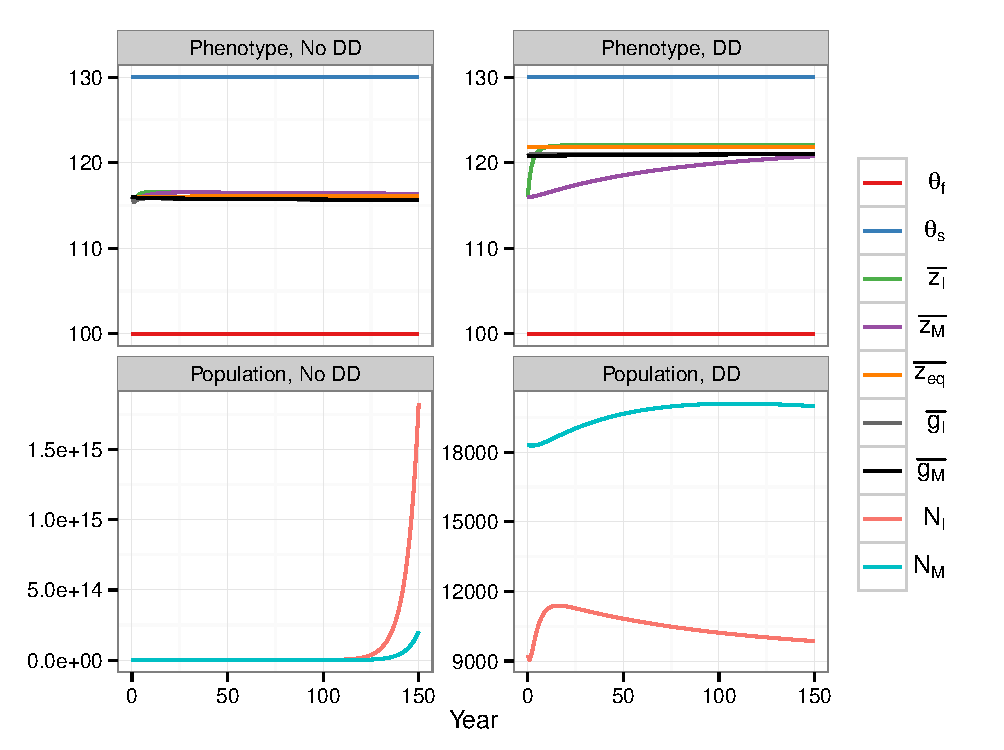
\includegraphics[scale=1]{Figures/DDphenopop.pdf}
	\caption{\textbf{Effect of density-dependence on phenotypes and populations}.}
	\label{fig:dd}
\end{figure}

\subsection*{Fluctuating optimums}

The noises were drawn from a bivariate normal distribution to make the optimums fluctuate. We varied the correlation between them.

\textbf{Figure2:} 3 panels, each with one value of noise correlation $\rho_{N}$ + $\overline{s_{I}}, \overline{f_{1}}, \overline{f_{2}}$/time with their values in constant environment.
\ref{fig:corr}

Explain in the text correlation of $z_{I}$ with $\theta_{s}(t)$

\begin{figure}[ht!]
	\centering
	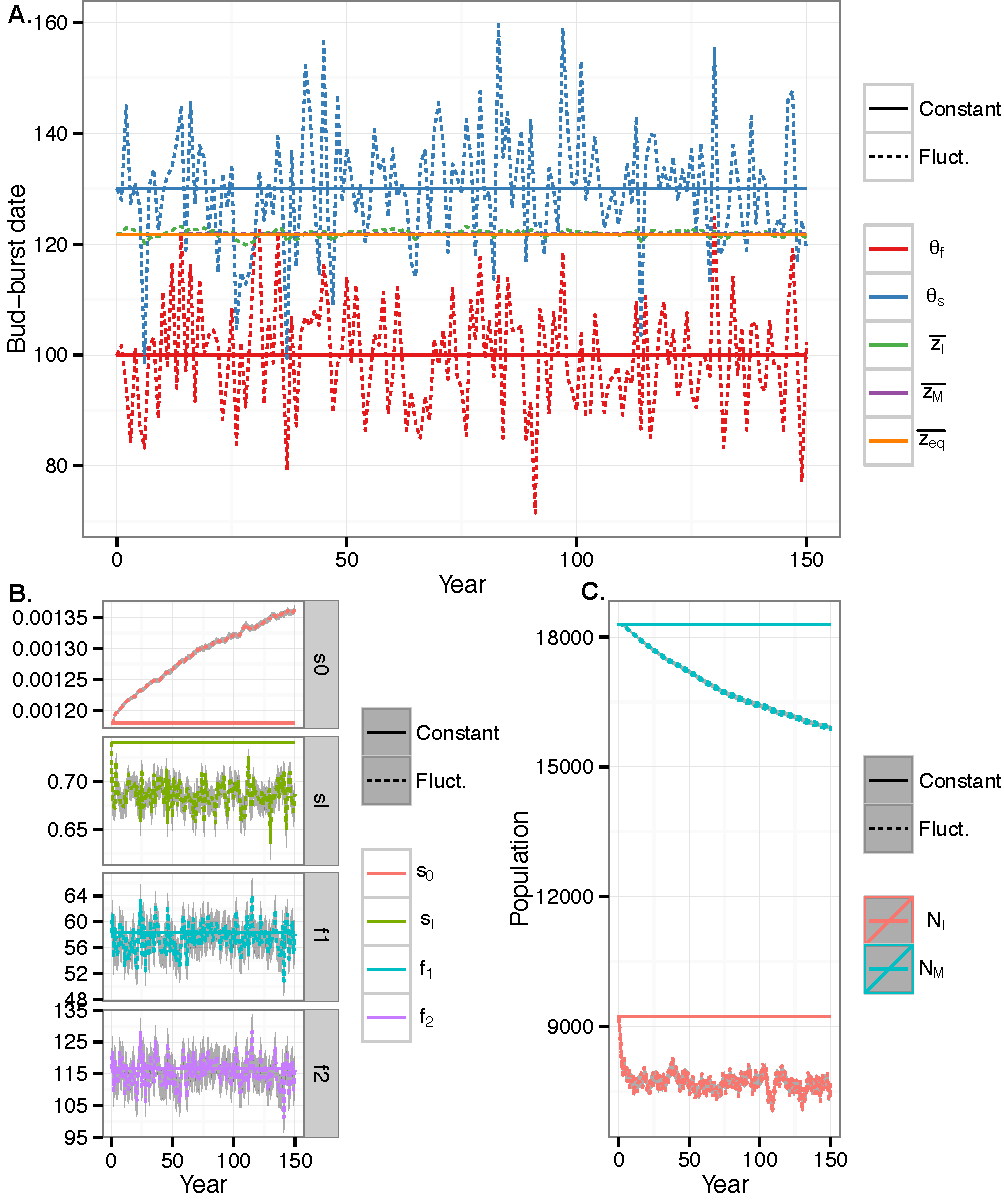
\includegraphics[scale=1]{Figures/PhenoLHTwithCorr.pdf}
	\caption{\textbf{Effect of the correlation of fluctuations on phenotypes and life-history traits}. Correlation coefficient $\rho_{N}$ values of noises are indicated on the top.}
	\label{fig:corr}
\end{figure}

\subsection*{Trend in the environment}

Decreasing optimums through time to mimic the advance in phenology with climate change.

\textbf{Figure:} Trend 2 panels with and without fluctuations, simulations results phenotype/time (with and without DD)

\subsection*{Estimation of the fluctuations}

\begin{figure}[ht!]
	\centering
	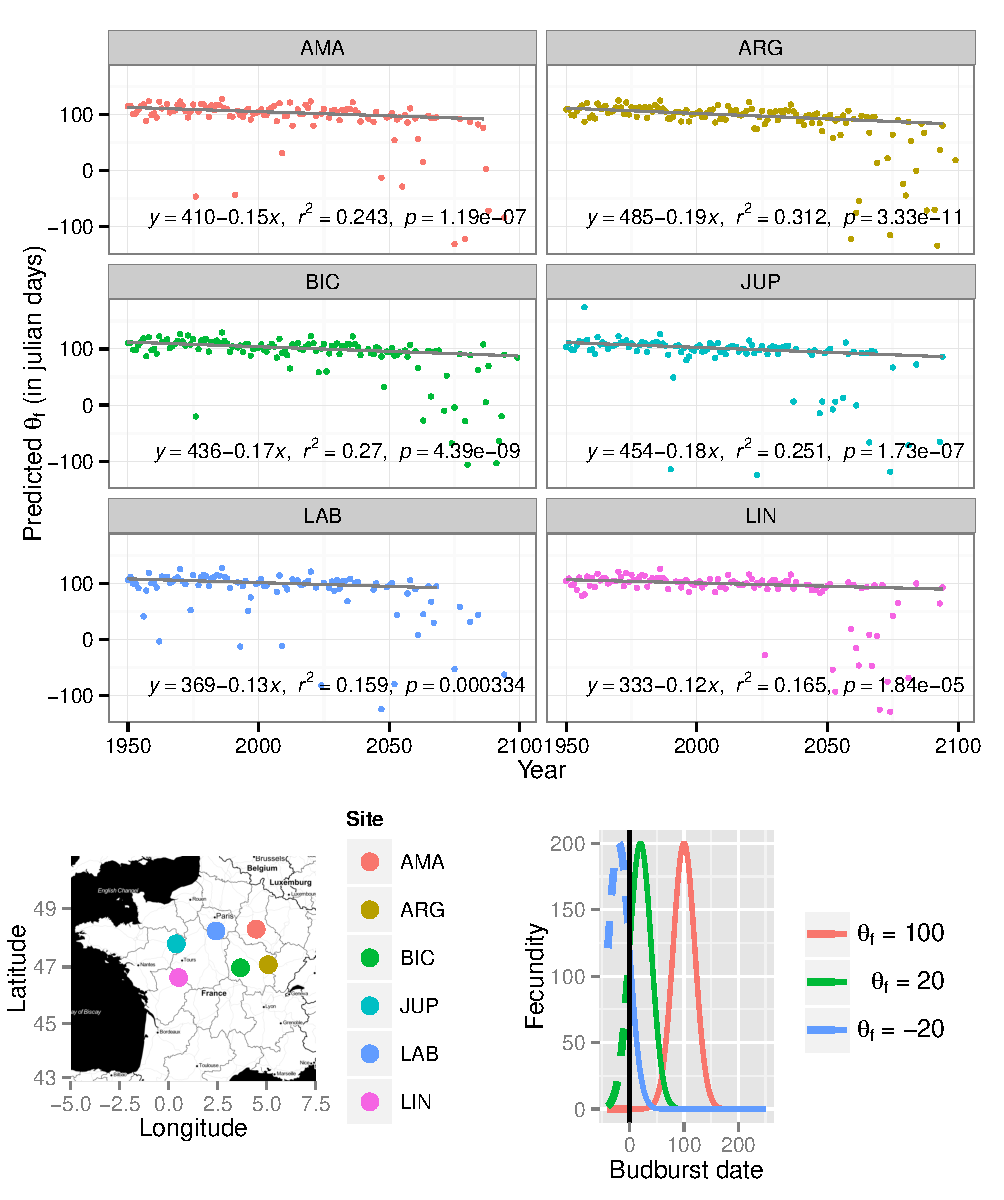
\includegraphics[scale=1]{Figures/optsmaps.pdf}
	\caption{\textbf{$\theta_{f}$ estimations from PHENOFIT data}.}
	\label{fig:thetaf}
\end{figure}

From phenofit.

\textbf{Figure:} Map of the localities, with panels for each of the optimums variations + graph showing fitness landscape with negative optimums

\textbf{Table:} table with slope and noise variance estimates for all years, years before 2001 (simulated climate close to real one), after 2001 (projection in climate evolution)